% Template for PLoS
% Version 2.0 July 2014
%
% To compile to pdf, run:
% latex plos.template
% bibtex plos.template
% latex plos.template
% latex plos.template
% dvipdf plos.template
%!TEX encoding = UTF-8 Unicode
% % % % % % % % % % % % % % % % % % % % % %
%
% -- IMPORTANT NOTE
%
% Be advised that this is merely a template 
% designed to facilitate accurate translation of manuscript content 
% into our production files. 
%
% This template contains extensive comments intended 
% to minimize problems and delays during our production 
% process. Please follow the template 
% whenever possible.
% % % % % % % % % % % % % % % % % % % % % % % 
%
% Once your paper is accepted for publication and enters production, 
% PLEASE REMOVE ALL TRACKED CHANGES in this file and leave only
% the final text of your manuscript.
%
% DO NOT ADD EXTRA PACKAGES TO THIS TEMPLATE unless absolutely necessary.
% Packages included in this template are intentionally
% limited and basic in order to reduce the possibility
% of issues during our production process.
%
% % % % % % % % % % % % % % % % % % % % % % %
%
% -- FIGURES AND TABLES
%
% DO NOT INCLUDE GRAPHICS IN YOUR MANUSCRIPT
% - Figures should be uploaded separately from your manuscript file. 
% - Figures generated using LaTeX should be extracted and removed from the PDF before submission. 
% - Figures containing multiple panels/subfigures must be combined into one image file before submission.
% See http://www.plosone.org/static/figureGuidelines for PLOS figure guidelines.
%
% Tables should be cell-based and may not contain:
% - tabs/spacing/line breaks within cells to alter layout
% - vertically-merged cells (no tabular environments within tabular environments, do not use \multirow)
% - colors, shading, or graphic objects
% See http://www.plosone.org/static/figureGuidelines#tables for table guidelines.
%
% For sideways tables, use the {rotating} package and use \begin{sidewaystable} instead of \begin{table} in the appropriate section. PLOS guidelines do not accomodate sideways figures.
%
% % % % % % % % % % % % % % % % % % % % % % % %
%
% -- EQUATIONS, MATH SYMBOLS, SUBSCRIPTS, AND SUPERSCRIPTS
%
% IMPORTANT
% Below are a few tips to help format your equations and other special characters according to our specifications. For more tips to help reduce the possibility of formatting errors during conversion, please see our LaTeX guidelines at http://www.plosone.org/static/latexGuidelines
%
% Please be sure to include all portions of an equation in the math environment, and for any superscripts or subscripts also include the base number/text. For example, use $mathrm{mm}^2$ instead of mm$^2$ (do not use the\textsuperscript command).
%
% DO NOT USE the \rm command to render mathmode characters in roman font, instead use $\mathrm{}$
% For bolding characters in mathmode, please use $\mathbf{}$ 
%
% Please add line breaks to long equations when possible in order to fit our 2-column layout. 
%
% For inline equations, please do not include punctuation within the math environment unless this is part of the equation.
%!TEX encoding = UTF-8 Unicode
% For spaces within the math environment please use the \; or \: commands, even within \text{} (do not use smaller spacing as this does not convert well).
%
%!TEX encoding = UTF-8 Unicode
% % % % % % % % % % % % % % % % % % % % % % % %



\documentclass[10pt]{article}
\usepackage{colortbl}
\usepackage{multirow}
% amsmath package, useful for mathematical formulas
\usepackage{amsmath}
% amssymb package, useful for mathematical symbols
\usepackage{amssymb}

% cite package, to clean up citations in the main text. Do not remove.
\usepackage{cite}
 
\usepackage{hyperref}

% line numbers
\usepackage{lineno}
 
 % ligatures disabled
\usepackage{microtype}
\usepackage{graphicx} 
 
% \DisableLigatures[f]{encoding = *, family = * }

% rotating package for sideways tables
%\usepackage{rotating}

% If you wish to include algorithms, please use one of the packages below. Also, please see the algorithm section of our LaTeX guidelines (http://www.plosone.org/static/latexGuidelines) for important information about required formatting.
%\usepackage{algorithmic}
%\usepackage{algorithmicx}

% Use doublespacing - comment out for single spacing
%\usepackage{setspace} 
%\doublespacing


% Text layout
\topmargin 0.0cm
\oddsidemargin 0.5cm
\evensidemargin 0.5cm
\textwidth 16cm 
\textheight 21cm

% Bold the 'Figure #' in the caption and separate it with a period
% Captions will be left justified
\usepackage[labelfont=bf,labelsep=period,justification=raggedright]{caption}
 
 % Remove brackets from numbering in List of References
\makeatletter
\renewcommand{\@biblabel}[1]{\quad#1.}
\makeatother


% Leave date blank
\date{}

\pagestyle{myheadings}

%% Include all macros below. Please limit the use of macros.

%% END MACROS SECTION

 
\begin{document}


% Title must be 150 characters or less
\begin{flushleft}
{\Large
\textbf{Evaluating Metagenome Assembly on a Complex Community}
}
% Insert Author names, affiliations and corresponding author email.
\\
 
Sherine Awad $^{1}$, 
Luiz Irber $^{1}$, 
C. Titus Brown $^{1,\ast}$ 

\bf{1} Population Health and Reproduction
University of California, Davis, Davis, CA, USA 
 
 
$\ast$ E-mail:  ctbrown@ucdavis.edu 
\end{flushleft}

% Please keep the abstract between 250 and 300 words
% Please keep the abstract between 250 and 300 words
\section*{Abstract}
NEEDS ENHANCEMENTS

Motivation: With the emergence of de novo assembly, several work have been to done to assemble metagenomic data from de novo. Several assemblers exist that are based on different assembly techniques. However, we still lack  a study that analyze different assemblers behavior on metagenomic data . 


Problem statement: In this paper, we performed analytical study for metagnome assembly using different assemblers and different preprocessing treatments. The aim of the analysis is studying how well metagenome assembly works, and which assembly works best. In addition, the study analyzes the resource requirements of the assembly. 


Approach: We used a mock community dataset for the analysis, and used its reference genome for benchmark evaluation. We quality filtered the reads, then we applied 2 other preprocessing steps: digital normalization and partitioning. We used 4 different assembler: Velvet, IDBA-UD, SPAdes, and MEGAHIT to assemble the reads using each treatment. We used QUAST to analyze assemblies accuracy. 
%@SAM let me show you something about IDBA-UD pls

Results: Results show that assembly works well. Velvet is the worst assembler in terms of accuracy and recourses utilizations. The results also showed that assembly counts to most of the reads. 
 
 
Conclusions: Except for Velvet, assemblers works well. Further analysis is required to study which assembler is better used with each specific dataset. This step is left for our future work, 
% Please keep the Author Summary between 150 and 200 words
% Use first person. PLOS ONE authors please skip this step. 
% Author Summary not valid for PLOS ONE submissions.   
\section*{Author Summary}

WHAT SHOULD BE WRITTEN HERE


\section*{Introduction}

 
Metagenome is the sequencing of DNA in an environmental sample. While whole genome sequencing (WGS) usually targets one genome, metagenome targets several ones which introduces complexity to metagenome analyis due to genomic diversity and variable abundance within populations.  Metagenomic assembly  means the assembly of multiple genomes from mixed sequences of reads of multiple species in a microbial community.  
Most approaches for analyzing metagenomic data rely on mapping to reference genomes. However, not all microbial diversity of many environments are covered by reference databases. Hence, the need for de novo assembly of complex metagenomic data rises.  
Several assemblers exist that can be used for de novo assembly. In order to decide which assembly works best, we need to evaluate metagenome assembly generated by each assembler.  In this paper, we provide, an evaluation for metegnome assembly generated by several assemblers and using different preprocessing treatments. We use a reference genome as a benchmark for the evaluation.  The evaluation is based on assembly accuracy, and time and memory requirements. This evaluation shed light on doability of metagenome assembly and the minimum requirements needed for the assembly. In addition, knowing how each assembler works, helps deciding which assembler to use prior to assembly. However, the later point is left for our future work. 
 
The comparative study in this paper is based on four different assemblers; Velvet \cite{velvet}, SPAdes \cite {spades}, IDBA-UD \cite{idba}, and MEGAHIT \cite{megahit}.  


Velvet \cite{velvet} is a group de Bruin graph-based sequence assembly methods for very short reads that can both remove errors. It also uses read pair information to resolve a large number of repeats.  The error correction algorithm merges the sequences that belongs together. Then the repeat solver algorithm separates parts that share overlaps. 


SPAdes \cite{spades} is an assembler for both single-cell and standard (multicell) assembly. SPAdes generates single-cell assemblies and provides information about genomes of uncultivatable bacteria that vastly exceeds what may be obtained via traditional metagenomics studies. 

IDBA-UD \cite{idba} is a de Bruijn graph approach for assembling reads from single cell sequencing or metagenomic sequencing technologies with uneven sequencing depths. IDBA-UD uses multiple depth-relative thresholds to remove erroneous k-mers in both low-depth and high-depth regions. It also uses paired-end information  to solve the branch problem of low-depth short repeat regions. It applies and error correction step to correct reads of high-depth regions that can be aligned to high confident contigs.

MEGAHIT \cite{megahit} is a new approach that constructs a succinct de Bruijn graph using multiple k-mers, and uses a novel "mercy k-mer" approach that preserves low-abundance regions of reads. It also uses GPUs to accelerate the graph construction.
 
%In the next sections, we present dataset used, preprocessing treatments,  results and discussion. 

% You may title this section "Methods" or "Models". 
% "Models" is not a valid title for PLoS ONE authors. However, PLoS ONE
% authors may use "Analysis" 
\section*{Materials and Methods}

\subsection*{Datasets}

We used a diverse mock community data set containing 64 known species,
sequenced with Illumina HiSeq, yielding 109,629,496 paired-end sequences with
an untrimmed length of 11.07 Gbp and an estimated insert size of $\sim$ 380
\cite{podar}.
% @CTB please move insert size estimate to results somewhere.

We received the reference genomes from the original authors
(posted on j) and the original reads are available through
the NCBI Sequence Read Archive at Accession SRX200676. Figure \ref{fig:coverage-profile} shows the coverage profile of the reference genome, and the percentage of read with that coverage.  
%@CTB The figure drawn is using quality filtered reads, will add another one for the raw reads. 

\subsection*{Quality Filtering} 

We removed adapters with Trimmomatic v0.30 in paired-end mode with the
Truseq adapters \cite{trim}.
%The command line options used was TruSeq3-PE.fa:2:30:10??: Cite note for Mircea Reply
 %@CTB - please find out what adapters we should use for trimming. It's
%probably not TruSeq3.
%@SAM what we used TruSeq3-PE.fa:2:30:10?? 
We next used the fastq\_quality\_filter %(@CTB what program exactly?)
from the FASTX-Toolkit v0.0.13.2 \cite{FXtoolkit} to remove sequences  %(@CTB describe what those parameters do)
using the parameters -Q33 -q 30 -p 50, which keeps all sequences with 50\% or more bases with quality score greater than or equal to 30. %where -q  is the minimum quality score to keep  and -p is the minimum percent of bases that must have [-q] quality and Q33 to set the right offset for Sanger quality scores.

 %(cite fastx, give version). 

\subsection*{Mapping}

We aligned all quality-filtered reads to the reference metagenome with bwa
aln (v0.7.7.r441) \cite{bwa}. % (@SAM people cite bwa or bwa mem can't find citation for bwa aln??)  %(XXX give version and any command line options thataren't default).
  We aligned paired-end and orphaned reads separately using bwa aln samse.
We then used
 samtools (v0.1.19 ) \cite{sam-stools} to convert SAM files to BAM files for both
paired-end and orphaned reads. To count the unaligned reads, we find the records with the ``4" flag in the SAM files \cite{sam-stools}. 

We found chimeric alignments with the bwa mem aligner using the
default parameters (v0.7.7.r441).  Chimeric alignments cut reads in
two (or more).  For each chimeric alignment, in the SAM file, there
will be a primary alignment and at least one secondary alignment
tagged SA.  To count the chimeric alignments, we count the records
with the ``SA" flag in the SAM file \cite{sam-stools}. 

To extract the reads that contribute to unaligned contigs, we mapped the quality filtered reads to the unaligned contigs using bwa aln (v0.7.7.r441) \cite{bwa}. 
Then we used samtools \cite{sam-stools} to retrieve the reads that are mapped to the unaligned contigs. 

\subsection*{Reference Coverage and Coverage Profile} 

To evaluate how much of the reference genome was contained in the read
data, we used bwa aln to map reads to the reference genome.
We then calculated how many
reference bases are contained in at least one mapped read (script {\tt
sam-calc-refcov-cmp.py}). 

\subsection*{Digital Normalization} 

We applied the {\tt normalize-by-median.py} script from khmer v1.1 to
execute abundance normalization (``digital normalization'', \cite{brown2012})  on the data, retaining paired reads and using a
k-mer size of 20 (-p -k 20).  We executed digital normalization with 4
hash tables, each 1 GB in size (-N 4 -x 1e9).  After read
normalization, we used the {\tt filter-abund.py} script to trim
high-abundance reads (estimated k-mer coverage $\geq$ 20) at low-abundance
k-mers (k-mer abundance $\leq$ 2)   %@CTB check these parameters) 
to remove erroneous k-mers  \cite{qingpeng2014} \cite{streaming}. 
%(@cite Zhang et al., 2014 PLoS One; Zhang et al.,2015 (peerJ)).
%@SAM what is zhang et al. peerJ 2015? 

%@CTB was a second round of digital normalization run here?
%@SAM yes, this is the second round

\subsection*{Partitioning} 

We next applied partitioning to the data \cite{jpell2012, ahowe2014}.
We first eliminated high-abundance k-mers that could join multiple
species bins using the {\tt filter-below-abund.py} script from khmer v1.1 using an abundance cutoff of 50 or higher.
We then ran {\tt do-partition.py} with a k-mer size of 32 and 4 Bloom
filters each of size 1 gigabit for partitioning (-k 32 -N 4 -x 1e9).  After
partitioning, partitions were extracted to groups using the {\tt extract-partitions.py} script with a maximum group size of 100,000 ({\tt -X 100000}).

\subsection*{Metagenomes Assembly and evaluation}

We assembled the reads using four different assemblers: Velvet \cite{velvet}, IDBA-UD \cite{idba}, SPAdes \cite{spades}, and MEGAHIT \cite{megahit}.

For Velvet v1.2.07  \cite{ velvet}, we used k-mer values from 19 to 51
incremented by 2. We also used -fastq.gz for fastq format,
-shortPaired for the pe files and -short for the se files. Also, we
asked Velvet to automatically calculate expected coverage and coverage
cutoff ({\tt -exp\_cov auto -cov\_cutoff auto}).
From among the many assemblies, one for each k-mer size,
we then chose the assembly that had the most bases in contigs longer than
500 bp (script {\tt calc-best-assembly.py}).

For IDBA-UD v1.1.1 \cite{idba},  we used  --pre\_correction to perform pre-correction before assembly and -r for the pe files. 
For SPAdes v3.1.1 \cite{spades}, we used --sc --pe1-12   where --sc is required for MDA (single-cell) data  and --pe1-12  for file with interlaced reads for the first paired-end library.%@SAM this is what we used? 

For MEGAHIT \cite{megahit}, we used -l 101 -m 3e9 --cpu-only where -l is for maximum read length , -m is for max memory in byte to be used, and --cpu-only to use CPU not GPU.

%Spades? YYYY
%Megahit? YYYY

We examined the assembly quality of each assembler and treatment using
QUAST v2.3 \cite{quast} using quast.py and we use the default minimum
contig length equal to 500.

% Results and Discussion can be combined.


\subsection*{Treating Ambiguous Mapping} 

We define ambiguous mapping as any base that maps to more than one position in the reference genome.  We used two approaches to dealing with ambiguous mapping: 
Best-hit and ambiguous approaches. In the best-hit approach, we  consider only the mapping that has high confidence and discard the other mapping completely, so every base in the reference genome is hit once or zero times.  In the ambiguous approach, we use all mapping, and whenever a base in the reference genome is hit more than one time, we count it's coverage once. 


\section*{Results}

\subsection*{Cost of Assembly} 
We estimated time and memory requirements for each of them. We also estimated the running time and memory utilization for each assembler under both treatments and compared to assemblers time and memory requirements using quality filtered reads.  

Digital normalization utilized 74.93 GB of memory and took around 3
hours and 53 minutes to run. Partitioning utilized 21.78 GB and around
2 hours and a half to run. %@ctb Luiz said he doesn't see anything wrong in the script

For Velvet assemblies, table \ref{table:time-memory} row 3, it took $\sim 60$ hours using quality filtered reads, while it took only $\sim 6$ hours using digital normalizations
and $\sim 4$ hours using partitioning.  For IDBA-UD assemblies, table \ref{table:time-memory} row 6, it took $\sim 33$ hours using quality filtered reads, while it took $\sim 6$
hours using digital normalization and $\sim 8$ hours using
partitioning.  SPAdes assemblies utilized $\sim 67$ hours using quality
filtered reads while it took $\sim15$ hours and $\sim 7$ hours using
digital normalization and partitioning respectively, table \ref{table:time-memory} row 9. Finally, for
MEGAHIT, it took $\sim 2$ hours, $\sim$ half an hour, and $\sim$ hour
and a half using quality-filtered reads, digital normalization, and
partitioning respectively, table \ref{table:time-memory} row 12.
 
For Velvet assemblies, table \ref{table:time-memory} row 4, it used 98.40 GB of memory using quality
filtered reads, while it used one 52.67 GB and 35.23 GB of memory when
applying digital normalization and partitioning respectively. For IDBA-UD
assemblies, table \ref{table:time-memory} row 7, it used used 123.84 GB of memory using quality filtered
reads, while it used one 99.88 GB and 76.53 GB of memory when applying
digital normalization and partitioning respectively. For SPAdes
assemblies, table \ref{table:time-memory} row 10, it used 381.79 GB of memory using quality filtered reads,
while it used one 121.52 GB and 94.70 GB of memory when applying
digital normalization and partitioning respectively.  For MEGAHIT, table \ref{table:time-memory} row 13 it
utilizes 33.41 GB, 18.89 GB, 13.17 GB for quality-filtered reads,
digital normalization, and partitioning respectively. See Table
\ref{table:time-memory} for more details. 


In terms of compute cost, Megahit is the fastest and utilizes less memory. 
In conclusion, quality filtering utilizes more resources digital normalization and the later utilizes more resources than partitioning.


\subsection*{Assembly Comparisons} 

%NEW RESULTS TO BE ADDED HERE 

\subsection*{Evaluation Against the Reference Genome} 


\subsection*{Assembly alignment} 
We aligned each assembly to the reference genome using nucmer {cite here}. The we used our script {analyze\_assembly.py} to analayze the results. 
IDBA quality filtered assembly has 27,444 contigs,  out of which 71.36 \% is totally aligned to the reference genome. For SPAdes quality filtered assembly, it has 33,704 contigs  and 72.22\% is totally aligned to the reference. Finally,  Megahit has 75,497 contigs and 74.97\% is totally aligned to the reference.

\subsection*{Read Incorporation}
To evaluate how much of the reads are captured by the assembly, we mapped the quality filtered reads to each assembly.  Then we extracted the unaligned sequences. 
%RERUN USING CONTIGS THAT ARE NOT ALIGNED AT ALL 



\subsection*{More about unalignments}
%\subsection*{The de novo assemblies recover unexpected genomic sequence from the mock community}

We extracted the reads that contributed to unaligned contigs of each assembler (see Methods:Mapping). We mapped those reads to the reference genome. We find that most of the reads that mapped to the unaligned contigs don't exist in the reference genome.  Figure \ref{fig:unaliged-hist} shows a histogram for the percentage of reads contributed to unaligned contigs (orange columns) and the portion of those reads that mapped to the reference genome (green columns). 
%SHERINE: script unaignment-analysis.sh is currently running for this under run directory 


\subsection*{More about misassemblies} 
We extracted all the partially aligned contigs. Using IDBA and quality filtering, 11.99\% of the contigs were partially aligned. 49.73\% of the partially aligned contigs has less than 50 bases only unaligned while 50.27\% has 50 bases or more unaligned. Using SPAdes and quality filtering, 10.82\% of the contigs were partially aligned. 51.44\%of the partially aligned contigs has less than 50 bases only unaligned while 48.56\% has 50 bases or more unaligned.
Using Megahit and quality filtering,  10.45\% of the contigs were partially aligned.  58.49\%of the partially aligned contigs has less than 50 bases only unaligned while 41.51\% has 50 bases or more unaligned.

 
\subsection*{More about uncovered regions}
 
We used the same scrit {} to analyze the uncovered regions. Approximately 2.02\% of the reference bases are uniquely covered by IDBA quality filtered assembly,  $\sim$9.75\% and  $\sim$6.54\% of the reference bases are uniquely covered by SPAdes and Megahit quality filtered assembly respectively using Besthit approach. 
Approximately   $\sim$10.60\% of reference bases are uniquely uncovered by IDBA quality filtered assembly,  $\sim$7.62\% and  $\sim$3.44\% of the reference bases are uniquely uncovered by SPAdes and Megahit quality filtered assemblies respectively using Besthit approach. Meanwhile, there are  31,446,810  ($\sim$15.29\%)  of the reference bases commonly uncovered by IDBA, SPAdes, and Megahit quality filtered assemblies. 

%SHERINE: uncovered.py script is being fixed and rerun to draw a coverage profile for common uncovered bases and results to be added here.

 
\subsection*{Subsambling}
%RE-RUN ANALYSIS USING OUR SCRIPT AND UPDATE HERE 

%ADD HERE HOW DID WE SAMPLE OR MOVE TO METHODS 

Using quality filtering treatment and 25\% coverage, we counted the genome coverage using both best-hit and ambiguous approaches. 
Using ambiguous approach, genome coverage is 77.38\%, 82.53\%, and 81.30\% and with duplication ratio 1.38\%, 1.24\%, and 1.26\% for IDBA, SPAdes, and Megahit respectively.
Using best-hit approach, genome coverage is  63.10\%, 70.6\%, and 71.75\%  and with duplication ratio 0.27\%, 0.40\%, and 0.34 \% for IDBA, SPAdes, and Megahit respectively.

%We need to repeat the same section for coverage 50, 75 % : prepare jobs for running 

\section*{Discussion}
 

\subsection*{Assembly works well} 
Much of the reference is covered by the assembly.
Most contigs are broadly accurate. (Q: How do we measure this?)
Most genes within the reference are recovered.
The assembly represents the majority of the reads (90\%?) and the majority of the k-mers (XX).

 
\section*{Acknowledgments}



% Either type in your references using
%\begin{thebibliography}{}
% \bibitem{brown12}
%C. Titus Brown and  Adina Howe and Qingpeng Zhang  and Alexis B. Pyrkosz and Timothy H. Brom, A Reference-Free Algorithm for Computational Normalization of Shotgun Sequencing Data
 %\end{thebibliography}
%
% OR
%
% Compile your BiBTeX database using our plos2009.bst
% style file and paste the contents of your .bbl file
% here.
% 


 % Use the PLoS provided BiBTeX style
\bibliographystyle{plos2009}
%--------Added by Sherine----------------------------------------------
\bibliography{References}

 %------------------------------------------------------------------------------
\section*{Figure Legends}
% This section is for figure legends only, do not include
% graphics in your manuscript file.
%
%\begin{figure}
%\caption
%{
%{\bf Bold the first sentence.}  Rest of figure caption.  
%}
%\label{Figure_label}
%\end{figure}
\begin{figure} [h] 
 
\begin{center}  
 

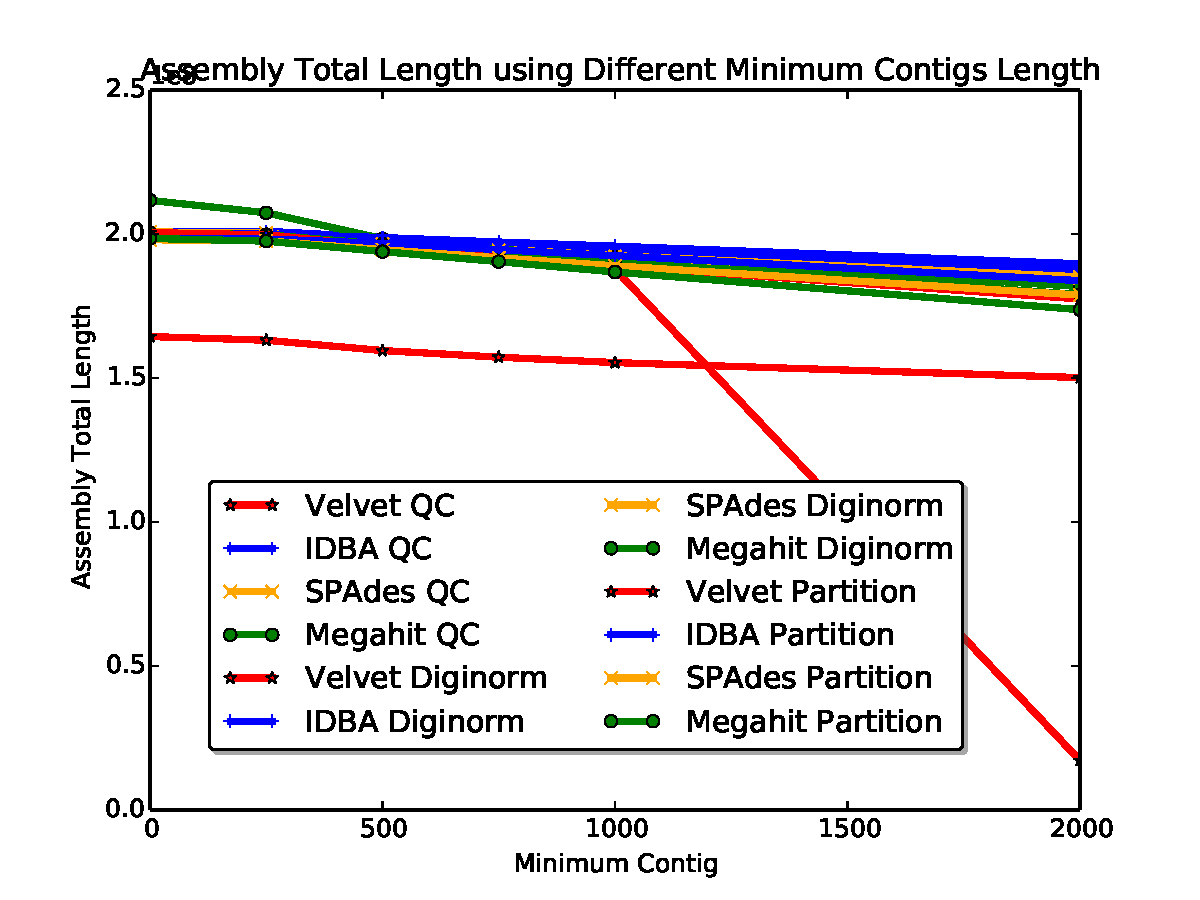
\includegraphics[height=3.2in,width=4.5in]{total-length-contigs.pdf}  
\caption{\small \sl Total Length of assemblies in basepairs based on different min contigs length.\label{fig:mincontig}}  
\end{center}  
\end{figure}  
 

\begin{figure} [h] 
\begin{center}  
 
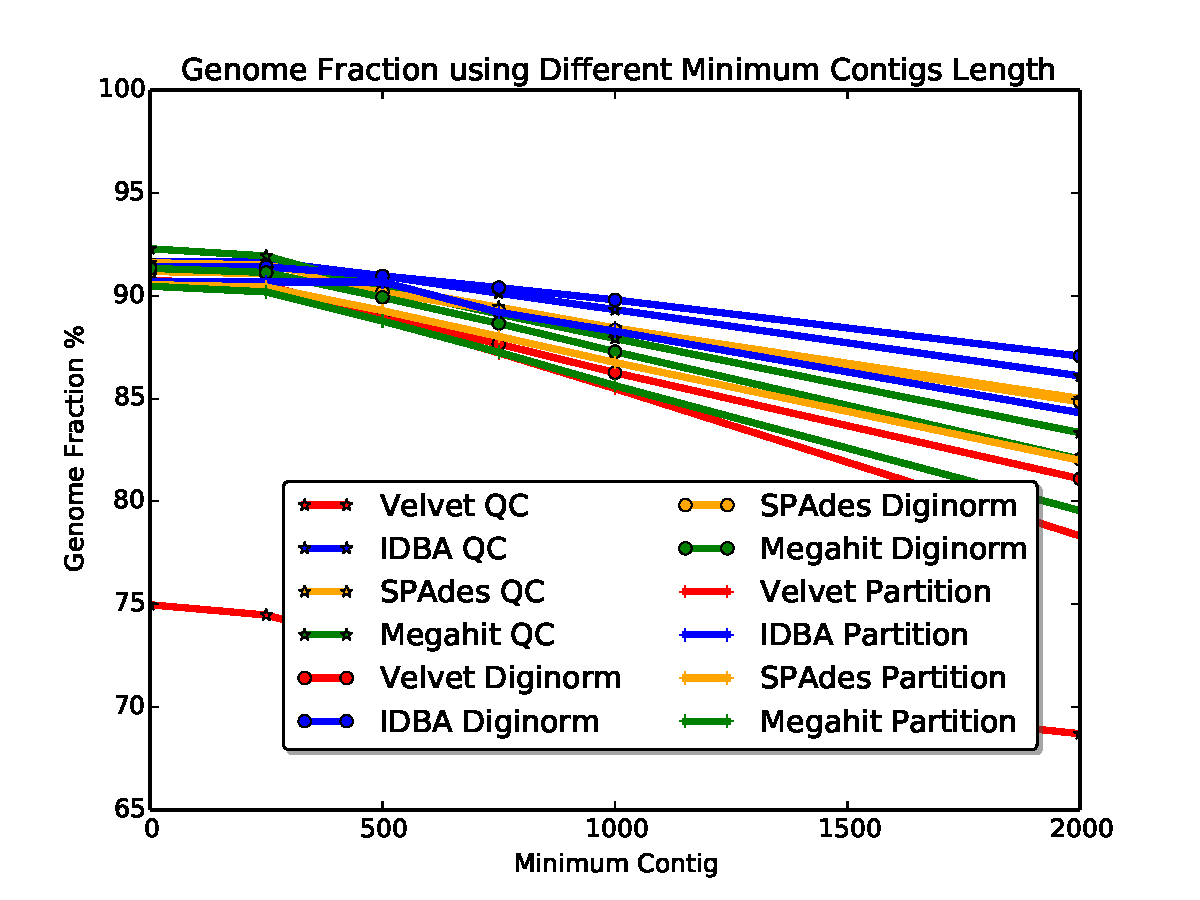
\includegraphics[height=3.2in,width=4.5in]{genome-fraction-contigs.pdf}  
\caption{\small \sl Genome Fraction of assemblies in basepairs based on different min contigs length.\label{fig:gf}}  
\end{center}  
\end{figure}  


\begin{figure} [h] 
\begin{center}  
 
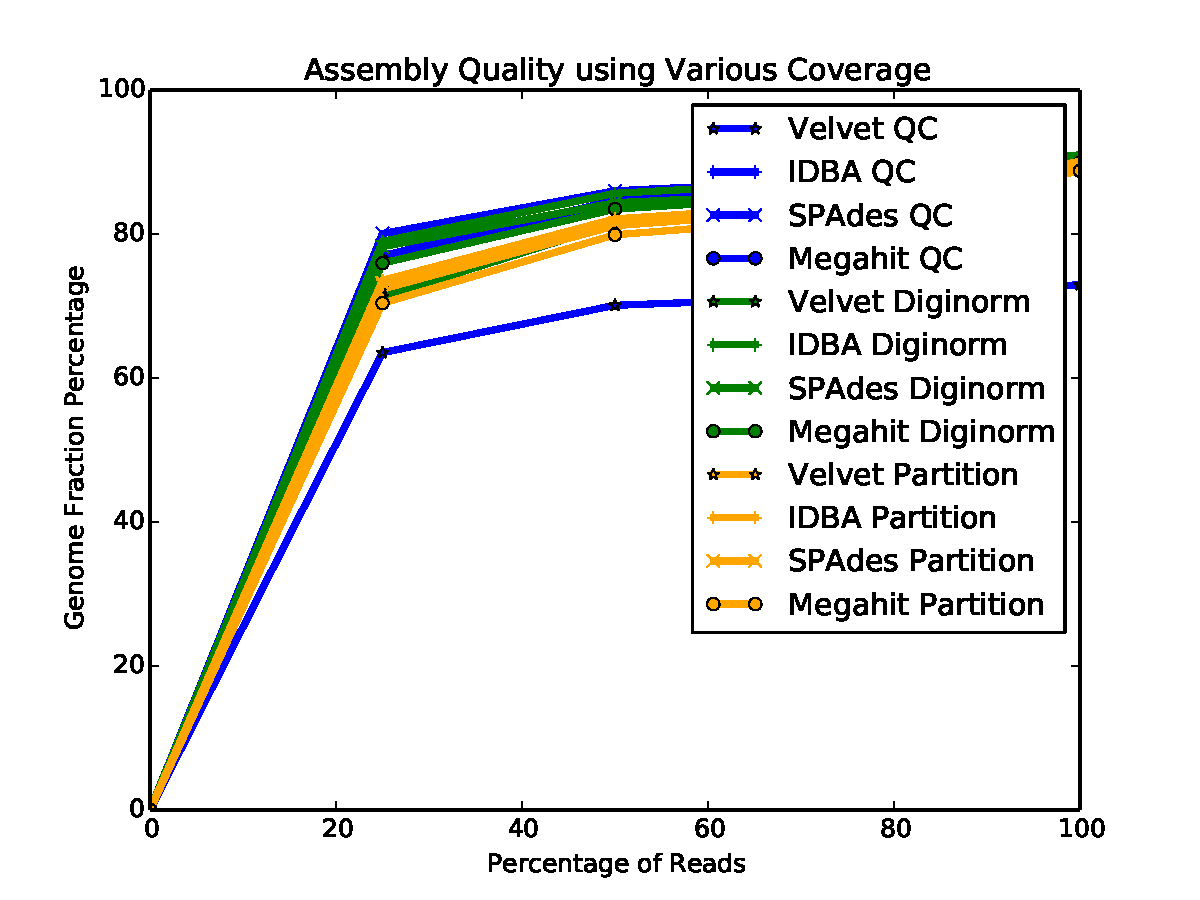
\includegraphics[height=3.2in,width=4.5in]{sampling.pdf}  
\caption{\small \sl Genome Fraction of assemblies using different read coverage.\label{fig:sampling}}  
\end{center}  
\end{figure}  
 

\begin{figure} [h] 
\begin{center}  
 
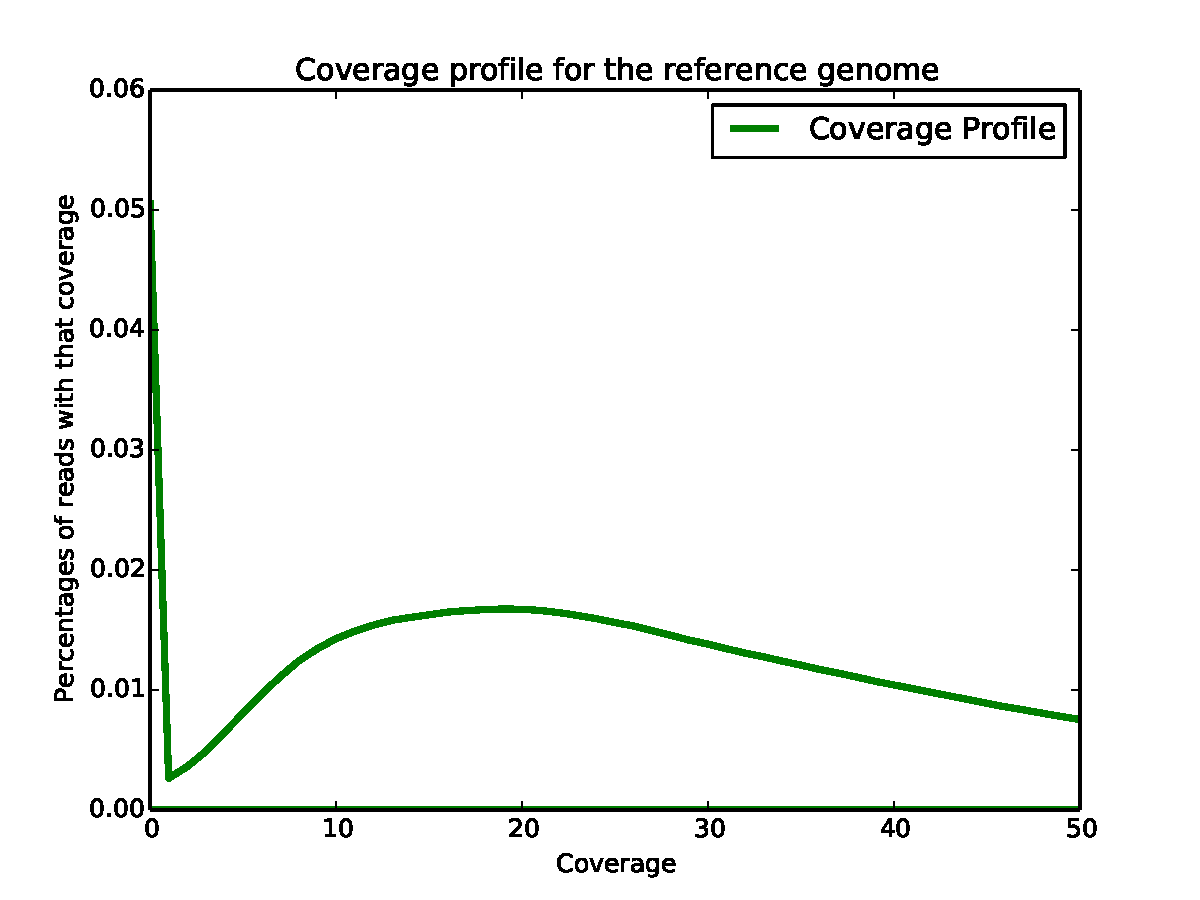
\includegraphics[height=3.2in,width=4.5in]{profilecoveragereads.pdf}  
\caption{\small \sl Reference genome coverage.\label{fig:coverage-profile}}  
\end{center}  
\end{figure} 


\begin{figure} [h] 
\begin{center}  
 
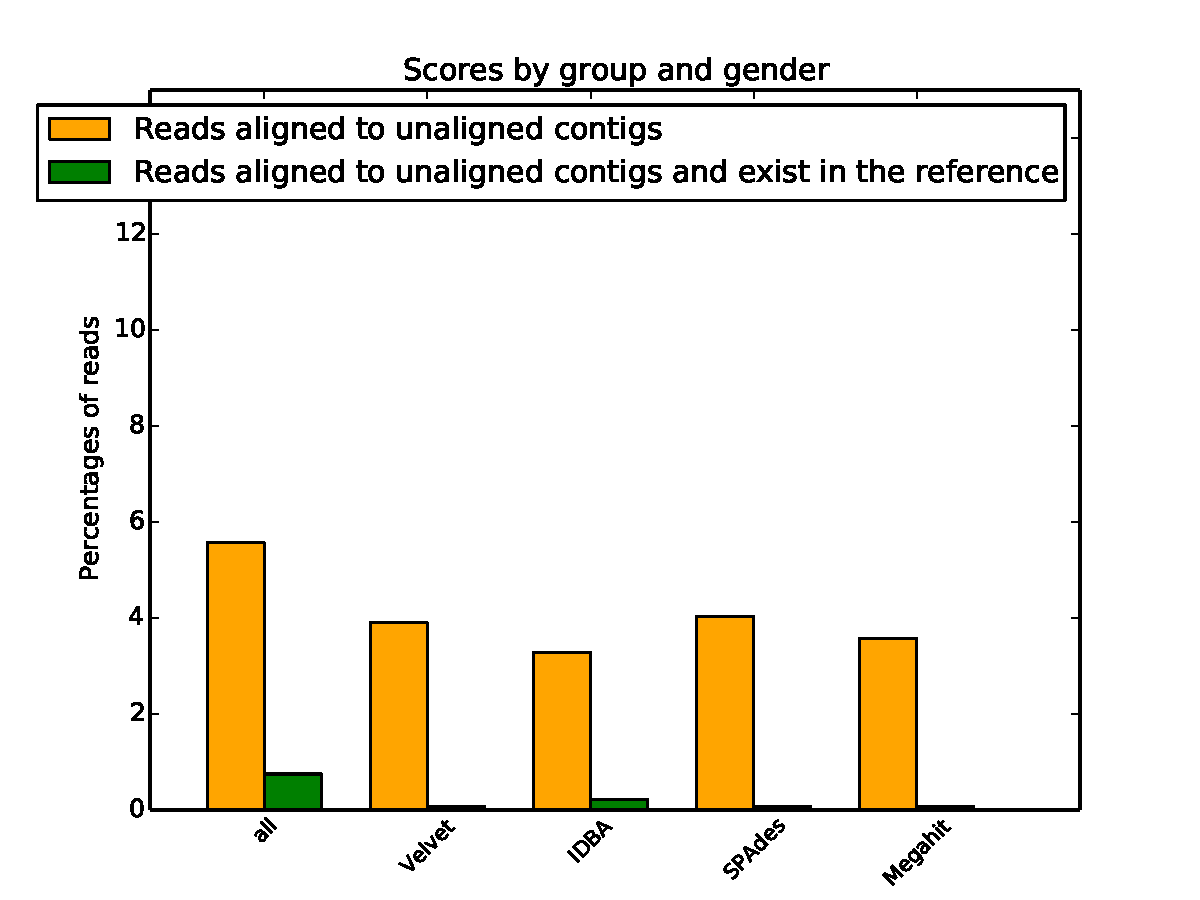
\includegraphics[height=3.2in,width=4.5in]{unaliged-hist.pdf}  
\caption{\small \sl Histogram for unaligned reads.\label{fig:unaliged-hist}}  
\end{center}  
\end{figure} 

\section*{Tables}
% 
% See introductory notes if you wish to include sideways tables.
%
% NOTE: Please look over our table guidelines at http://www.plosone.org/static/figureGuidelines#tables to make sure that your tables meet our requirements. Certain types of spacing, cell merging, and other formatting tricks may have unintended results and will be returned for revision.
%
%\begin{table}[!ht]
%\caption{
%\bf{Table title}}
%\begin{tabular}{|c|c|c|}
%table information
%\end{tabular}
%\begin{flushleft}Table caption
%\end{flushleft}
%\label{tab:label}
% \end{table}








%\begin{table}[t]
%\caption{Coverage Distribution}
%\centering
%\begin{tabular}{|c|c|}
%\hline
% \textbf{Coverage Range}& \textbf{No. of Reads}   \\ [0.5ex] % inserts table %heading
%\hline
%{ Between 20 and 40} & 95,540,661 \\
%\hline
%{ Between 40 and 60} &108,083 \\
%\hline
%{ Between 60 and 80} &22,677\\
%\hline
%{ Between 80 and 100} &17,148\\
%\hline
%{ Between 100 and 200} &80,878\\
%\hline
%{Coverage $\geq 200$} & 402,333\\
%\hline
%\end{tabular}
%\label{table:cov-dist} 
%\end{table}



\begin{table}[h]
\caption{Reference Genome Coverage and Duplication Ratio}
\centering
\begin{tabular}{|c|c|c|c|c|c|}
\hline
\textbf {Minimum IDY}&\textbf {Treatment/Quality Metric}& \textbf{Quality Filtering} & \textbf{Digital Normalization} & \textbf{Partition} &\\ [0.5ex] % inserts table %heading
\hline 
 \multicolumn{5}{|c|} {\textbf{(1) BEST HIT APPROACH}}    \\ [0.5ex] % inserts table %heading
\hline
\multicolumn{5}{|c|}{ \textbf{(1) IDBA-UD}}    \\ [0.5ex] % inserts table %heading
\hline
\multirow{2}{*}{99.0}&\textbf{Genome  Coverage\%} &57.81\%&&    \\   
&\textbf{Duplication Ratio} &0.49&  &   \\   
\hline
\multirow{2}{*}{95.0}&\textbf{Genome  Coverage\%} & 59.11\%&&    \\   
&\textbf{Duplication Ratio}&0.78&  &   \\   
\hline
\multicolumn{5}{|c|}{ \textbf{(2) SPAdes} }   \\ [0.5ex] % inserts table %heading
\hline
\multirow{2}{*}{99.0}&\textbf{Genome Coverage\%} &68.52\%& && \\
&\textbf{Duplication Ratio} &0.38 && & \\   
\hline
\multirow{2}{*}{95.0}&\textbf{Genome Coverage\%} &70.00 \%& && \\
&\textbf{Duplication Ratio} & 0.52&	 & & \\   
\hline
\multicolumn{5}{|c|}{ \textbf{(3) MEGAHIT} }    \\ [0.5ex] % inserts table %heading
\hline
\multirow{2}{*}{99.0}&\textbf{Genome  Coverage\%}&69.50\% & && \\
&\textbf{Duplication Ratio} &4.25&	 & & \\   
\hline
\multirow{2}{*}{95.0}&\textbf{Genome  Coverage\%}&70.99\% & && \\
&\textbf{Duplication Ratio} &4.70&	 & & \\   
\hline
 \multicolumn{5}{|c|} {\textbf{(2) AMBIGUOUS APPROACH}}    \\ [0.5ex] % inserts table %heading
\hline
\multicolumn{5}{|c|}{ \textbf{(1) IDBA-UD}}    \\ [0.5ex] % inserts table %heading
\hline
\multirow{2}{*}{99.0}&\textbf{Genome  Coverage\%} &89.56\%&	 &&  \\   
&\textbf{Duplication Ratio} &1.05&	& &  \\   
\hline
\multirow{2}{*}{95.0}&\textbf{Genome  Coverage\%} &95.47\%&	 &&  \\   
&\textbf{Duplication Ratio} &2.30&	& &  \\   
\hline
\multicolumn{5}{|c|}{ \textbf{(2) SPAdes} }   \\ [0.5ex] % inserts table %heading
\hline
\multirow{2}{*}{99.0}&\textbf{Genome Coverage\%}&89.49\% & & &\\
&\textbf{Duplication Ratio} &0.99&	 & & \\   
\hline
\multirow{2}{*}{95.0}&\textbf{Genome Coverage\%}& 96.11\% & & &\\
&\textbf{Duplication Ratio} &1.58&	 & & \\   
\hline
\multicolumn{5}{|c|}{ \textbf{(3) MEGAHIT} }    \\ [0.5ex] % inserts table %heading
\hline
\multirow{2}{*}{99.0}&\textbf{Genome Coverage\%} &90.60\% & &  &\\
&\textbf{Duplication Ratio} &5.04&	 &&  \\   
\hline
\multirow{2}{*}{95.0}&\textbf{Genome Coverage\%} &95.85\% & &  &\\
&\textbf{Duplication Ratio} &6.73&	 &&  \\   
\hline
\end{tabular}
\label{table:coverage-analysis}
\end{table}


\begin{table}[h]
\caption{Contigs Analysis}
\centering
\begin{tabular}{|c|c|c|c|c|}
\hline
\textbf {Treatment/Quality Metric}& \textbf{Quality Filtering} & \textbf{Digital Normalization} & \textbf{Partition} \\ [0.5ex] % inserts table %heading
\hline 
 \multicolumn{4}{|c|} {\textbf{(1) BEST HIT APPROACH}}    \\ [0.5ex] % inserts table %heading
 \hline
\multicolumn{4}{|c|}{ \textbf{(1) IDBA-UD}}    \\ [0.5ex] % inserts table %heading
\hline
\textbf{No. of Contigs} &27,444&&    \\   
\hline
\textbf{Totally Aligned Contigs \%} &71.36\% &  &   \\   
\hline
\textbf{Partial Aligned Contigs \%} &11.99\% &  &   \\   
\hline
\textbf{Unaligned Contigs \%} &16.65\% &  &   \\   
\hline
\multicolumn{4}{|c|}{ \textbf{(2) SPAdes} }   \\ [0.5ex] % inserts table %heading
\hline
\textbf{No. of Contigs}&33,704&&    \\   
\hline
\textbf{Totally Aligned Contigs\%} &72.22\% &  &   \\   
\hline
\textbf{Partial Aligned Contigs\%} &10.82\%&  &   \\   
\hline
\textbf{Unaligned Contigs\%}&16.96\% &  &   \\   
\hline
\multicolumn{4}{|c|}{ \textbf{(3) MEGAHIT} }    \\ [0.5ex] % inserts table %heading
\hline
\textbf{No. of Contigs} &75,497&&    \\   
\hline
\textbf{Totally Aligned Contigs \%} &74.97\%&  &   \\   
\hline
\textbf{Partial Aligned Contigs\%} &10.45\%&  &   \\   
\hline
\textbf{Unaligned Contigs\%}&14.58\%&  &   \\   
\hline
\multicolumn{4}{|c|} {\textbf{(2) AMBIGUOUS  APPROACH}}    \\ [0.5ex] % inserts table %heading
\hline
\multicolumn{4}{|c|}{ \textbf{(1) IDBA-UD}}    \\ [0.5ex] % inserts table %heading
\hline
\textbf{No. of Contigs} &27,444&&    \\   
\hline
\textbf{Totally Aligned Contigs\%}&77.56\%&  &   \\   
\hline
\textbf{Partial Aligned Contigs\%}&10.15\%&  &   \\   
\hline
\textbf{Unaligned Contigs \%}&12.28\%&  &   \\   
\hline
\multicolumn{4}{|c|}{ \textbf{(2) SPAdes} }   \\ [0.5ex] % inserts table %heading
\hline
\textbf{No. of Contigs} &33,704&&    \\   
\hline
\textbf{Totally Aligned Contigs} &75.65\%&  &   \\   
\hline
\textbf{Partial Aligned Contigs\%}&8.12\%&  &   \\   
\hline
\textbf{Unaligned Contigs\%}&16.23\%&  &   \\   
\hline
\multicolumn{4}{|c|}{ \textbf{(3) MEGAHIT} }    \\ [0.5ex] % inserts table %heading
\hline
\textbf{No. of Contigs}&75,497&&    \\   
\hline
\textbf{Totally Aligned Contigs\%} &78.20\%&  &   \\   
\hline
\textbf{Partial Aligned Contigs\%}&9.22\%&  &   \\   
\hline
\textbf{Unaligned Contigs\%}&12.58\% &  &   \\   
\hline
\end{tabular}
\label{table:contigs-analysis}
\end{table}


\begin{table}[h]
\caption{More Coverage Analysis}
\centering
\begin{tabular}{|c|c|c|c|c|}
\hline
\textbf {Treatment/Quality Metric}& \textbf{Quality Filtering} & \textbf{Digital Normalization} & \textbf{Partition} \\ [0.5ex] % inserts table %heading
\hline 
 \multicolumn{4}{|c|} {\textbf{(1) BEST HIT APPROACH}}    \\ [0.5ex] % inserts table %heading
\hline
\multicolumn{4}{|c|}{ \textbf{(1) IDBA-UD}}    \\ [0.5ex] % inserts table %heading
\hline
\textbf{Uniquely Covered\%}&2.02\%&&    \\   
\hline
\textbf{Uniquely Uncovered}&10.60\%&  &   \\   
\hline
\multicolumn{4}{|c|}{ \textbf{(2) SPAdes} }   \\ [0.5ex] % inserts table %heading
\hline
\textbf{Uniquely Covered\%}&9.75\%& & \\
\hline
\textbf{Uniquely Uncovered\%}&7.62\%&	 &  \\   
\hline
\multicolumn{4}{|c|}{ \textbf{(3) MEGAHIT} }    \\ [0.5ex] % inserts table %heading
\hline
\textbf{Uniquely Covered\%}&6.54\%& & \\
\hline
\textbf{Uniquely Uncovered\%}& 3.44\%&	 &  \\   
\hline
 \multicolumn{4}{|c|} {\textbf{(2) AMBIGUOUS APPROACH}}    \\ [0.5ex] % inserts table %heading
\hline
\multicolumn{4}{|c|}{ \textbf{(1) IDBA-UD}}    \\ [0.5ex] % inserts table %heading
\hline
\textbf{Uniquely Covered\%}&0.88\%& & \\
\hline
\textbf{Uniquely Uncovered\%}&1.62\%&	 &  \\   
\hline
\multicolumn{4}{|c|}{ \textbf{(2) SPAdes} }   \\ [0.5ex] % inserts table %heading
\hline
\textbf{Uniquely Covered\%}&0.99\%& & \\
\hline
\textbf{Uniquely Uncovered\%}&1.81\%&	 &  \\   
\hline
\multicolumn{4}{|c|}{ \textbf{(3) MEGAHIT} }    \\ [0.5ex] % inserts table %heading
\hline
\textbf{Uniquely Covered\%}&1.52\%& & \\
\hline
\textbf{Uniquely Uncovered\%}&1.22\%&	 &  \\   
\hline
\end{tabular}
\label{table:coverage-analysis}
\end{table}



 



\begin{table}[h]
\caption{Running Time and Memory Utilization}
\centering
\begin{tabular}{|c|c|c|c| }
\hline
\textbf {Treatment/Quality Metric}& \textbf{Quality Filtering} & \textbf{Digital Normalization} & \textbf{Partition}  \\ [0.5ex] % inserts table %heading
\hline
 \multicolumn{4}{|c|} {\textbf{(1) Velvet}}    \\ [0.5ex] % inserts table %heading
\hline
\textbf{Running Time} &60:42:52 &6:48:46 &4:30:36   \\ 
\hline
\textbf{Memory Utilization in GB}&98.40&52.67&35.23\\ 
\hline
\multicolumn{4}{|c|}{ \textbf{(2) IDBA-UD}}    \\ [0.5ex] % inserts table %heading
\hline
\textbf{Running Time} &33:53:46&6:34:24 &8:30:29  \\ 
\hline`
\textbf{Memory Utilization in GB}&123.84&99.88&89.25\\ 
\hline
\multicolumn{4}{|c|}{ \textbf{(3) SPADes} }   \\ [0.5ex] % inserts table %heading
\hline
\textbf{Running Time} &67:02:16&15:53:10&7:54:26  \\
\hline
\textbf{Memory Utilization in GB}&381.79&121.52&123.7 \\ 
\hline
\multicolumn{4}{|c|}{ \textbf{(4) MEGAHIT} }    \\ [0.5ex] % inserts table %heading
\hline
\textbf{Running Time}&1:52:55&0:30:23&1:23:28 \\
\hline
\textbf{Memory Utilization in GB}&33.41&18.89&189.55 \\ 
\hline


\end{tabular}
\label{table:time-memory}
\end{table}



 
\begin{table}[t]
\caption{Comparision between N50 and NG50}
\centering
\begin{tabular}{|c|c|c|c|}
\hline
\textbf {Treatment}& \textbf{Quality Filtering} & \textbf{Digital Normalization} & \textbf{Partition}  \\ [0.5ex] % inserts table %heading
\hline
 \multicolumn{4}{|c|} {\textbf{(2) IDBA-UD}}    \\ [0.5ex] % inserts table %heading
\hline
\textbf{N50}&49,773&47,828&26,575 \\ 
\hline
\textbf{NG50}&45,748&44,351&24,326 \\
\hline
 \multicolumn{4}{|c|} {\textbf{(3) SPAdes}}    \\ [0.5ex] % inserts table %heading
\hline
\textbf{N50}&42,773&35,580&22,319\\ 
\hline
\textbf{NG50}&38,841&32,598&19,909\\
\hline
 \multicolumn{4}{|c|} {\textbf{(4) MEGAHIT}}    \\ [0.5ex] % inserts table %heading
\hline
\textbf{N50}&35,136&27,302&17,492\\ 
\hline
\textbf{NG50}&32,251&25,248&15,393\\
\hline
\end{tabular}
\label{table:n50-ng50} 
\end{table}




 \section *{Supporting Information Legends} 
%
% Please enter your Supporting Information captions below in the following format:
%\item{\bf Figure SX. Enter mandatory title here.} Enter optional descriptive information here.
% 
%\begin{description}
%\item {\bf}
%\item {\bf}
%\end{description}

\end{document}

